\PassOptionsToPackage{unicode=true}{hyperref} % options for packages loaded elsewhere
\PassOptionsToPackage{hyphens}{url}
\PassOptionsToPackage{dvipsnames,svgnames*,x11names*}{xcolor}
%
\documentclass[]{article}
\usepackage{lmodern}
\usepackage{amssymb,amsmath}
\usepackage{ifxetex,ifluatex}
\usepackage{fixltx2e} % provides \textsubscript
\ifnum 0\ifxetex 1\fi\ifluatex 1\fi=0 % if pdftex
  \usepackage[T1]{fontenc}
  \usepackage[utf8]{inputenc}
  \usepackage{textcomp} % provides euro and other symbols
\else % if luatex or xelatex
  \usepackage{unicode-math}
  \defaultfontfeatures{Ligatures=TeX,Scale=MatchLowercase}
\fi
% use upquote if available, for straight quotes in verbatim environments
\IfFileExists{upquote.sty}{\usepackage{upquote}}{}
% use microtype if available
\IfFileExists{microtype.sty}{%
\usepackage[]{microtype}
\UseMicrotypeSet[protrusion]{basicmath} % disable protrusion for tt fonts
}{}
\IfFileExists{parskip.sty}{%
\usepackage{parskip}
}{% else
\setlength{\parindent}{0pt}
\setlength{\parskip}{6pt plus 2pt minus 1pt}
}
\usepackage{xcolor}
\usepackage{hyperref}
\hypersetup{
            pdftitle={Amplified Oracle: Probably Better Methods for Rewarding Forecasters},
            pdfauthor={Nuño Sempere},
            colorlinks=true,
            linkcolor=Maroon,
            filecolor=Maroon,
            citecolor=Blue,
            urlcolor=blue,
            breaklinks=true}
\urlstyle{same}  % don't use monospace font for urls
\usepackage{graphicx,grffile}
\makeatletter
\def\maxwidth{\ifdim\Gin@nat@width>\linewidth\linewidth\else\Gin@nat@width\fi}
\def\maxheight{\ifdim\Gin@nat@height>\textheight\textheight\else\Gin@nat@height\fi}
\makeatother
% Scale images if necessary, so that they will not overflow the page
% margins by default, and it is still possible to overwrite the defaults
% using explicit options in \includegraphics[width, height, ...]{}
\setkeys{Gin}{width=\maxwidth,height=\maxheight,keepaspectratio}
\setlength{\emergencystretch}{3em}  % prevent overfull lines
\providecommand{\tightlist}{%
  \setlength{\itemsep}{0pt}\setlength{\parskip}{0pt}}
\setcounter{secnumdepth}{0}
% Redefines (sub)paragraphs to behave more like sections
\ifx\paragraph\undefined\else
\let\oldparagraph\paragraph
\renewcommand{\paragraph}[1]{\oldparagraph{#1}\mbox{}}
\fi
\ifx\subparagraph\undefined\else
\let\oldsubparagraph\subparagraph
\renewcommand{\subparagraph}[1]{\oldsubparagraph{#1}\mbox{}}
\fi

% set default figure placement to htbp
\makeatletter
\def\fps@figure{htbp}
\makeatother


\title{Amplified Oracle: Probably Better Methods for Rewarding Forecasters}
\author{Nuño Sempere\footnote{Quantified Uncertainty Research Institute.}}
\date{\today}

\begin{document}
\maketitle

\hypertarget{motivation}{%
\section{Motivation}\label{motivation}}

In \href{https://arxiv.org/abs/2106.11248}{Alignment Problems With
Current Forecasting Platforms}, Sempere and Lawsen outline a variety of
problems with current forecasting platforms, whose scoring rules are
found to either not be proper---as in the case of Good Judgment Open or
CSET-Foretell (now INFER)---or incentivize distorting one's true
probabilities to maximize the chances of placing in the top few
positions which earn a monetary reward---as in the case of Metaculus. In
addition, in almost all cases, forecasting platforms---or, for that
matter, prediction markets---disincentivize collaboration.

Against that backdrop,
\href{https://papers.ssrn.com/sol3/papers.cfm?abstract_id=3954498}{Reciprocal
Scoring: A Method for Forecasting Unanswerable Questions}, Karger et
al.~describe a method to elicit predictions in situations in which
resolutions are outright not possible, or very far away. They provide
some preliminary evidence of its effectiveness in the form of a small
randomized trial. However, in the post-peer-review discussion phase in
social media, Karger et al.'s method was met with an extremely lukewarm
reception from the community of forecasting practitioners, which has
grown to view methods which resemble Keynesian Beauty Constests with
suspicion.

In this working paper, we outline an alternative incentivization method,
an ``amplified oracle'', which roughly looks as follows:

\begin{itemize}
\tightlist
\item
  There is a trusted authority which cares about its long-term
  reputation. This central authority is trusted, but has limited
  capacity.
\item
  Forecasters are then rewarded according to a scheme where they
  forecast on all questions, the central authority predicts on only a
  few questions chosen randomly, and then forecasters are rewarded
  according to the proximity of their predictions to that central
  authority.
\end{itemize}

Towards the middle of the paper, we also point out that the ``central
authority'' doesn't have to be particularly privileged or more trusted
than the rest; the core feature is rather that some forecasters predict
other forecasters and the second group of forecasters predicts reality.

This scheme has the advantage that forecasters can be rewarded speedily
for questions which either have no objective resolution or happen far in
the future. In addition, if the trusted authority has long horizons, it
can be rewarded when the question resolves in the future, or according
to the best guess of a future forecasting system.

\hypertarget{description-of-the-method}{%
\section{Description of the method}\label{description-of-the-method}}

In the interest of brevity, we shall outline our method by means of an
example, and the example shall be the question ``Will the People's
Republic of China have annexed at least half of Taiwan by 2050?'', as
operationalized by
\href{https://www.metaculus.com/questions/5320/chinese-annexation-of-most-of-taiwan-by-2050/}{Metaculus}.
Alas, this method requires a cluster or questions, so the reader should
picture a cluster of questions similar to that one.

\hypertarget{the-oracle-determines-a-rough-prior-of-all-questios-in-order-to-reduce-potential-reward.}{%
\subsection{The oracle determines a rough prior of all questios, in
order to reduce potential
reward.}\label{the-oracle-determines-a-rough-prior-of-all-questios-in-order-to-reduce-potential-reward.}}

Taiwan has been independent of mainland China since the 25th of October
1945, i.e., 76 years into the past. Per Laplace's law, the chances that
this will change by 2050 is
\(1-(1-\frac{1}{(2021-1945)+2})^{2050-2021} \approx 31\%\). Lets take
this \(32\%\) as 's initial probability. Note that per the
\href{https://en.wikipedia.org/wiki/Reference_class_problem}{reference
class problem}, other reference classes might have been chosen, so the
point of this prior is not to be definitive, but rather to provide a
starting point less arbitrary than 50\% from which forecaster reward
might be computed in the next steps. In the case of a patron aiming to
learn from sponsoring a forecasting tournament, the prior might
represent the patron's initial probability.

\hypertarget{forecasters-attempt-to-foresee-the-oracles-future-forecast.}{%
\subsection{Forecasters attempt to foresee the oracle's future
forecast.}\label{forecasters-attempt-to-foresee-the-oracles-future-forecast.}}

Forecasters spend some effort trying to come up with forecasts which
beat the prior. If they are rewarded in proportion to how much they beat
this prior, as outlined in \href{}{Paying for bits}, they have an
incentive to collaborate.

\hypertarget{the-oracle-predicts-on-a-randomly-chosen-number-of-questions}{%
\subsection{The oracle predicts on a randomly chosen number of
questions}\label{the-oracle-predicts-on-a-randomly-chosen-number-of-questions}}

The oracle chooses some questions at random, and produces a forecast for
these questions.

\hypertarget{forecasters-are-rewarded-or-punished-according-to-how-much-their-probability-moves-from-the-prior-to-the-oracle-forecast.}{%
\subsection{Forecasters are rewarded or punished according to how much
their probability moves from the prior to the oracle
forecast.}\label{forecasters-are-rewarded-or-punished-according-to-how-much-their-probability-moves-from-the-prior-to-the-oracle-forecast.}}

As outlined in \href{}{Paying for bits}\footnote{Though this proposal
  can also be trivially adapted for use with other scoring rules.},
forecasters end up with a positive balance, if they have moved the
probability from the prior towards the oracle's forecast. But if they
moved the probability in the opposite direction, they end up with a
negative balance.

In this case, forecasters should be rewarded in proportion to the number
of questions which resolve. For instance, if the oracle only looks at
one in ten questions, reward or punishment is multiplied by 10.

Within the prediction market conceptualization, the maximum price of a
share would be \$10 rather than \$1. But since shares only have a 10\%
chance of paying out, their price doesn't exceed \$1.

\hypertarget{after-a-time-the-oracle-is-rewarded-or-punished}{%
\subsection{After a time, the oracle is rewarded or
punished}\label{after-a-time-the-oracle-is-rewarded-or-punished}}

Optionally, after a time, reality is observed, and the oracle itself is
paid or punished in proportion to their accuracy. But straight-out
rewards require the oracle to have relatively long time horizons, and
for anthropic effects to not hold (e.g., predicting a solar flare that
ends life has the feature that if you're wrong, you are already dead).

Alternatively, the oracle can itself be predicting the output of a more
thorough investigation. For instance, in the presence of a fair lottery,
that investigation can be made very intense and resource intensive with
a small probability for relatively little cost.

As a third option, the oracle may instead attempt to predict the
client's forecast after additional time has passed and more information
about the matter of interest has surfaced. In this case, it wouldn't be
that the client is a worse forecaster than the oracle, but just busier.

Readers may notice that this proposal resembles previously proposed
amplification setups, such as those in
\href{https://www.lesswrong.com/posts/cLtdcxu9E4noRSons}{Lagerros et
al.}, which themselves build on ideas by Paul Christiano.

\hypertarget{discussion-of-the-method}{%
\section{Discussion of the method}\label{discussion-of-the-method}}

\hypertarget{more-on-the-central-authority}{%
\subsection{More on the central
authority}\label{more-on-the-central-authority}}

Implicitly, we have been presenting this central authority as more
trustworthy, or more truth-seeking than the other forecasters which are
used to amplify it. But this might not necessarily be the case at all:
this method might be used as a cost-saving device instead. For instance,
maybe some forecasters are more willing to receive rewards later rather
than immediately, but both sets of forecasters produce similar quality
forecasts. Alternatively, perhaps all forecasters have similar discount
rates, but rewarding many forecasters for predictions which will be
resolved long into the future might be too expensive. In that case,
tournament designers might arbitrarily divide a tournament's cohort into
forecasters rewarded now and authorities which are rewarded later, with
the former attempting to predict and give information to the latter.

Note that this amplification method might go very wrong if forecasting
something such as ``Will the US dollar suffer from large amounts of
inflation?''. In that case, forecasters' who have reason to believe in
inflation might self-select into the group which gets rewarded now (in
dollars), and likewise forecasters with beliefs about lack of inflation
might self-select into the group which gets rewards later. In that case,
the first group of short-termists might sneakily predict that the second
group will think that there will be no inflation, but the link between
the forecasting system and reality would have been weakened.

\hypertarget{evidence-base-and-comparison-to-karger-et-al.s-method}{%
\subsection{Evidence base and comparison to Karger et al.'s
method}\label{evidence-base-and-comparison-to-karger-et-al.s-method}}

Most of the reasons why I think why this method might be superior come
from first principles reasoning or from my experience with forecasting.
With regards to first-principle reasoning, both steps of the system are
incentive compatible, and rational actors would thus be incentivized to
predict reality.

With regards to evidence from my experience as a forecaster, it just
feels more grounded. A first group of forecasters try to predict or
amplify a more patient group of forecasters, and the second group tries
to predict reality. If a forecaster has unique information, they can and
should try to convince the second group. If the evidence is just very
private or hard to communicate, the forecaster with that information
could offer a bet to the Bayesian approximator. Forecasters are
incentivized to conduct expensive searches (e.g., interviews with
citizens of far-away lands),
cf.~\href{https://twitter.com/LinchZhang/status/1455759586158268417}{Linch
Zhang}.

\begin{figure}
\centering
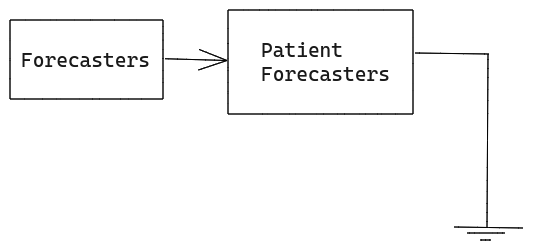
\includegraphics[width=0.5\textwidth,height=\textheight]{diagrams/amplify-samotsvety-1.png}
\caption{Proposed design}
\end{figure}

\begin{figure}
\centering
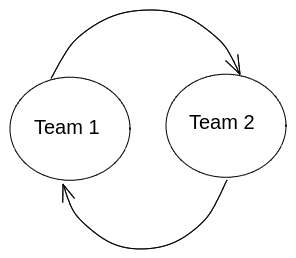
\includegraphics[width=0.3\textwidth,height=\textheight]{diagrams/karger-method.png}
\caption{Karger et al.'s design}
\end{figure}

In contrast, Karger et al.'s method has weird loops; teams are not
aiming to forecast reality, but rather to forecast what the other team
will forecast that one's team will forecast that the other team will
forecast\ldots{} In the presence of Schelling points, human biases,
laziness, etc., it is not clear that this process converges to the
truth. For instance, the forecaster which puts in the most research
effort, or the group which puts in the most effort, is disadvantaged:
ideally, both groups want to put in the same amount of effort, or,
equivalently, find out the same things. This is particularly egregious
when a forecaster has some piece of evidence that they don't expect
anybody on the other team to have. In that case, in Karger et al.'s
schema, the forecaster with unique knowledge may want to forecast as if
she did not know it.

Some of the authors in Karger et al.'s paper bring forward the argument
that if one has large enough teams, each person should expect and
equivalent someone in the other team to find the same evidence. Although
perhaps true in the limit, this in my experience does not seem likely to
be true in any degree of practice.

Karger et al.'s method has the advantage that it produces a legible
output, e.g., a wiki. In our case, the first group of forecasters might
use similar infrastructure when predicting the forecasts from the second
group, and the second group might use that infrastructure to organize
its own thoughts. So that doesn't seem like a unique advantage of Karger
et al.'s methods.

\hypertarget{conclusion}{%
\subsection{Conclusion}\label{conclusion}}

In conclusion, the proposed method of amplifying an perhaps more
expensive and powerful but perhaps just more patient group of
forecasters has the benefit of appearing more grounded, and not having
the weird loops in Karger et al.'s reciprocal scoring proposal---or in
other Keynesian beauty contest designs. We look forward to someone
trying to implement it.

\end{document}
